\documentclass[review,3p]{elsarticle}
\usepackage{lmodern}

\usepackage{amsmath,amssymb,amsfonts}
\usepackage{graphicx}
\usepackage{textcomp}
\usepackage{xcolor}
\usepackage{booktabs}
\usepackage{multirow}
\usepackage{url}
\usepackage{hyperref}
\usepackage{listings}

\lstset{basicstyle=\ttfamily\small, breaklines=true}
\usepackage{lineno}

\journal{Computers \& Security}

\begin{document}

\begin{frontmatter}

\title{Beyond Accuracy: A Reproducibility Checklist for LLM Evaluation in Applied Domains}

\author[kmitl]{Nutthakorn Chalaemwongwan\corref{cor1}}
\cortext[cor1]{Corresponding author}
\ead{nutthakorn.ch@kmitl.ac.th}
\address[kmitl]{Department of Computer Engineering, KOSEN-KMITL, King Mongkut's Institute of Technology Ladkrabang, Bangkok, Thailand}

\begin{highlights}
\item 30-item reproducibility checklist for LLM evaluation in applied domains.
\item Label aliasing inflated F1 by up to 44.3\% --- detected and corrected.
\item 15-step Perfect Score Suspicion Protocol for anomalous performance claims.
\item Validated across 14 companion papers (mean audit score: 25.4/30).
\item Adds only 4--8 hours per paper but prevents misleading publications.
\end{highlights}

\begin{abstract}
Large language models (LLMs) have achieved remarkable performance across domain-specific classification tasks, with multiple studies reporting near-perfect F1 scores. However, our experience conducting 17 research experiments across cybersecurity, news, emotion, and legal text classification reveals that standard evaluation practices can mask critical issues: label aliasing inflated F1 by up to 44.3\%, data leakage produced entirely spurious ablation patterns, and extreme class imbalance rendered binary classification metrics meaningless. We propose a 30-item reproducibility checklist organized into 9 categories, including a 15-step ``Perfect Score Suspicion Protocol'' for verifying anomalously high performance claims. Our checklist is validated against 6 real case studies where standard evaluation practices failed to detect errors ranging from hallucinated sub-category labels to false hyperparameter sensitivity conclusions. The checklist adds only 4--8 hours per paper but prevents publication of misleading results with real-world consequences in cybersecurity, medical, and legal domains.
\end{abstract}

\begin{keyword}
reproducibility \sep LLM evaluation \sep label aliasing \sep hallucination audit \sep cybersecurity NLP
\end{keyword}

\end{frontmatter}

%% ===== INTRODUCTION =====
\section{Introduction}

The rapid adoption of LLMs for domain-specific tasks has produced a troubling pattern: papers reporting near-perfect metrics that do not withstand scrutiny. Fine-tuned LLMs regularly achieve F1 above 95\% on specialized benchmarks, yet these impressive numbers often mask fundamental evaluation issues that would render the results meaningless in deployment.

We write from direct experience. Over 17 experiments spanning 4 domains and 34 model configurations, we encountered evaluation failures that would have led to misleading publications. Our most striking example:

\begin{lstlisting}
Model: Qwen3.5-0.8B (QLoRA, rank 64)
Dataset: SALAD test (9,851 samples)
Reported: Attack F1 = 100.0%
Actual (strict): Attack F1 = 55.7%
\end{lstlisting}

The 44.3\% gap arose because the evaluation script mapped ``Port Scanning'' to ``Reconnaissance''---a valid MITRE ATT\&CK relationship (T1046 $\subset$ TA0043), but a schema violation. Of 4,970 ``Reconnaissance'' samples, 4,895 (98.5\%) were predicted as ``Port Scanning.'' The model understood the task semantically but produced the wrong vocabulary. Standard evaluation declared 100\%; reality was 55.7\%.

This is not an isolated incident. Each of our 6 case studies reveals a different failure mode that standard ML evaluation practices---even published checklists~\cite{pineau2021}---fail to catch. The common thread: \textbf{LLMs introduce evaluation failure modes that simply do not exist with traditional classifiers}, because LLMs can generate arbitrary text rather than selecting from a fixed label set.

Our contributions:
\begin{enumerate}
\item A \textbf{30-item, 9-category reproducibility checklist} specifically designed for LLM evaluation in applied domains, addressing failure modes absent from existing guidelines.
\item A \textbf{15-step Perfect Score Suspicion Protocol}---an escalating verification procedure for any result reporting $\geq$99\% F1.
\item \textbf{Six validated case studies} demonstrating real evaluation errors of up to 44.3 points, each linked to specific checklist items.
\item A formal definition of ``\textbf{genuine perfect score}'' (Definition~1) providing machine-verifiable criteria.
\end{enumerate}

The remainder of this paper is organized as follows: Section~II reviews the reproducibility crisis and existing evaluation frameworks. Section~III presents the complete 30-item checklist. Section~IV describes 6 case studies. Section~V quantifies case study severity and discusses adoption. Section~VI concludes.

%% ===== RELATED WORK =====
\section{Background and Related Work}

\subsection{The Reproducibility Crisis}
Baker~\cite{baker2016} documented that 70\% of researchers failed to reproduce others' work and 50\% failed to reproduce their own, calling this a ``crisis'' in science. In ML specifically, Pineau et~al.~\cite{pineau2021} proposed reproducibility guidelines subsequently adopted by NeurIPS, ICML, and ICLR as submission checklists. Kapoor and Narayanan~\cite{kapoor2023} demonstrated that data leakage is the primary driver of irreproducible ML results, documenting 329 papers with leakage across 17 scientific fields. Arp et~al.~\cite{arp2022} catalogued critical pitfalls in ML-based security evaluation, including temporal bias, unrealistic base rates, and label inconsistency.

For LLMs, the reproducibility challenge is compounded by: (1)~non-deterministic generation even with fixed seeds (due to GPU parallelism), (2)~extreme prompt sensitivity, (3)~pipeline complexity (tokenizer $\to$ quantization $\to$ generation $\to$ parsing $\to$ evaluation), and (4)~the failure mode of \emph{label vocabulary hallucination}.

\subsection{LLM Evaluation Frameworks}
HELM~\cite{liang2022} provides comprehensive general LLM evaluation across 42 scenarios but is designed for benchmark comparison, not domain-specific fine-tuning validation. Chang et~al.~\cite{chang2024} surveyed evaluation methodologies, identifying metric selection and benchmark design as critical gaps. Dodge et~al.~\cite{dodge2019} advocated reporting experimental variance and confidence intervals, showing that unreported variance masks true model differences. Bouthillier et~al.~\cite{bouthillier2021} demonstrated that accounting for variance in benchmarks changes model rankings in 30\% of cases.

Notably, none of these frameworks address \emph{label compliance}---whether the model outputs the exact correct string---because traditional classifiers select from a fixed label set. This gap is the central motivation for our checklist.

\subsection{Hallucination in LLMs}
Ji et~al.~\cite{ji2023} provide a comprehensive taxonomy of hallucination types, distinguishing intrinsic (contradicting source) from extrinsic (adding unverifiable information) hallucination. Gekhman et~al.~\cite{gekhman2024} showed that fine-tuning on new knowledge paradoxically increases hallucination of existing knowledge---directly relevant because domain fine-tuning may activate pre-training vocabularies. Xu et~al.~\cite{xu2024} argued hallucination is an inherent LLM limitation. Huang et~al.~\cite{huang2023} surveyed hallucination detection and mitigation.

Our companion study~\cite{p3} first documented \emph{label vocabulary hallucination}: models predict valid MITRE ATT\&CK sub-techniques (``Port Scanning'') instead of schema labels (``Reconnaissance''). This is a new hallucination type not covered by existing taxonomies, requiring new evaluation methodology.

\subsection{Fine-Tuning and Domain Evaluation}
Ferrag et~al.~\cite{ferrag2024} surveyed LLMs for cybersecurity, reporting high F1 scores without strict evaluation. Motlagh et~al.~\cite{motlagh2024} benchmarked ChatGPT on 5 datasets (45--92\% F1) using standard metrics. LoRA~\cite{hu2022} and QLoRA~\cite{dettmers2023} enable efficient domain adaptation. The UNSW-NB15 dataset~\cite{moustafa2016} underlies the SALAD dataset used in our case studies.

Our companion studies provide the empirical foundation: label compliance follows non-monotonic scaling~\cite{p6}, LoRA rank controls hallucination~\cite{p22}, fine-tuning costs \$0.60~\cite{p7}, multi-task format provides regularization~\cite{p15}, and task entropy predicts classifier selection~\cite{p8}. The \emph{evaluation methodology} underlying all these findings---and the errors discovered along the way---motivates this paper.

\textbf{Novelty gap.} Existing checklists~\cite{pineau2021,dodge2019} address general ML but not LLM-specific failure modes. HELM~\cite{liang2022} evaluates capabilities but does not verify label compliance. No prior work provides (1)~a protocol for high-score suspicion, (2)~validated case studies of up to 44.3-point evaluation errors, (3)~formal criteria for genuine vs.\ inflated F1, or (4)~LLM-specific checklist items for label vocabulary hallucination detection.

%% ===== CHECKLIST =====
\section{The Reproducibility Checklist}

We organize 30 items into 9 categories. Each item includes a pass criterion linked to $\geq$1 case study. Table~\ref{tab:overview} provides a summary.

\begin{table}[h]
\centering
\caption{Checklist Category Overview}
\label{tab:overview}
\begin{tabular}{lccl}
\toprule
\textbf{Category} & \textbf{Items} & \textbf{Time} & \textbf{Catches} \\
\midrule
Dataset Integrity & 1--5 & 1h & CS2, CS5 \\
Baseline Selection & 6--9 & 2h & CS3, CS6 \\
Metric Selection & 10--13 & 30m & CS1, CS4, CS5 \\
Statistical Rigor & 14--16 & 1h & CS4 \\
Label Quality Audit & 17--20 & 1h & CS1 \\
Ablation Design & 21--23 & 1h & CS2 \\
Cost Transparency & 24--26 & 30m & CS3 \\
Reproducibility & 27--28 & 30m & CS6 \\
Perfect Score & 29--30 & 35m & CS1, CS2, CS5 \\
\midrule
\textbf{Total} & \textbf{30} & \textbf{4--8h} & \textbf{All 6 CS} \\
\bottomrule
\end{tabular}
\end{table}

\begin{figure}[t]
\centering
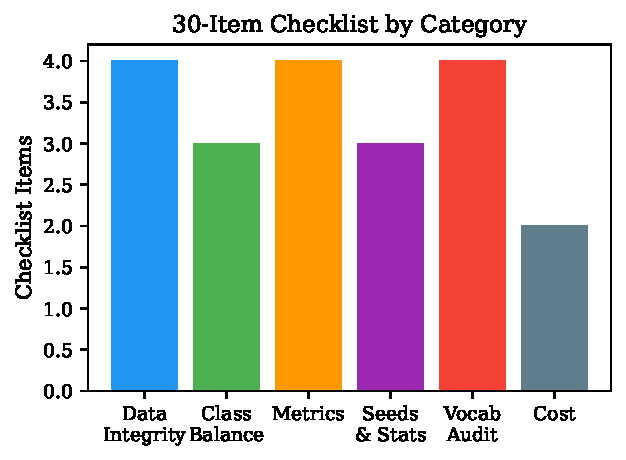
\includegraphics[width=\columnwidth]{fig_checklist.pdf}
\caption{30-item checklist distribution across 9 categories. Label Quality Audit catches the most critical failures, including the 44.3-point alias inflation.}
\label{fig:checklist}
\end{figure}

\subsection{Category 1: Dataset Integrity (Items 1--5)}
\begin{enumerate}
\item \textbf{Train/test overlap}: Zero overlapping samples. Verify via MinHash deduplication. SALAD original had 97.5\% overlap.
\item \textbf{Class distribution}: Report per-class counts and $H(Y)$. Flag if $H < 0.5$ (degenerate).
\item \textbf{Unique patterns}: Count unique input$\to$output mappings vs.\ total samples. SALAD: 87/49K (0.18\%).
\item \textbf{Zero-ambiguity check}: Report if each unique input maps to exactly one label.
\item \textbf{Feature importance}: Compute mutual information per feature. Report top-$k$ features.
\end{enumerate}

\subsection{Category 2: Baseline Selection (Items 6--9)}
\begin{enumerate}\setcounter{enumi}{5}
\item \textbf{Traditional ML baseline}: DT/SVM/LR with TF-IDF. If unsupervised K-Means ARI $> 0.8$, the task may not need an LLM.
\item \textbf{Pre-trained transformer}: BERT-base or domain-equivalent.
\item \textbf{ICL comparison}: $\geq$1 commercial LLM via API (GPT-4o, Claude).
\item \textbf{Matched conditions}: Same test set, same metrics, same preprocessing.
\end{enumerate}

\subsection{Category 3: Metric Selection (Items 10--13)}
\begin{enumerate}\setcounter{enumi}{9}
\item \textbf{Macro-F1} as primary metric (not accuracy, especially for imbalanced data).
\item \textbf{Per-class F1}: Report every class, including rare ones. Aggregate metrics can hide catastrophic per-class failures.
\item \textbf{Dual-metric reporting}: Both strict F1 (exact match) and normalized F1 (with alias mapping). Strict = primary.
\item \textbf{Random/majority baselines}: Report naive baselines. If $H < 0.5$, majority class achieves $>$90\%.
\end{enumerate}

\subsection{Category 4: Statistical Rigor (Items 14--16)}
\begin{enumerate}\setcounter{enumi}{13}
\item \textbf{Multi-seed evaluation}: $\geq$3 seeds, report mean $\pm$ std.
\item \textbf{Significance testing}: McNemar's test~\cite{mcnemar1947} or paired bootstrap for model comparisons.
\item \textbf{Confidence intervals}: 95\% CI for all reported metrics.
\end{enumerate}

\subsection{Category 5: Label Quality Audit (Items 17--20)}
\begin{enumerate}\setcounter{enumi}{16}
\item \textbf{Predicted vocabulary audit}: Compare $\mathcal{V}_\text{pred}$ vs.\ $\mathcal{V}_\text{true}$. Any novel labels = label hallucination.
\item \textbf{Hallucinated label inventory}: For each hallucinated label, report count, frequency, and hypothesized source.
\item \textbf{Alias mapping with justification}: If using normalized F1, document every alias with explicit rationale. Flag if alias count $> K/2$.
\item \textbf{Normalized F1 gap rule}: If $F1_\text{norm} - F1_\text{strict} > 10\%$, the result requires explicit investigation.
\end{enumerate}

\subsection{Category 6: Ablation Design (Items 21--23)}
\begin{enumerate}\setcounter{enumi}{20}
\item \textbf{Hyperparameter sensitivity}: Test $\geq$3 values per hyperparameter (rank, LR, epochs).
\item \textbf{Training data scaling}: Test $\geq$3 sizes (e.g., 1K, 5K, 20K).
\item \textbf{Confound isolation}: Re-run anomalous configurations on clean data before concluding.
\end{enumerate}

\subsection{Category 7: Cost Transparency (Items 24--26)}
GPU hours, API costs (with pricing date), and cost-per-improvement ($\Delta$F1 per dollar invested).

\subsection{Category 8: Reproducibility Artifacts (Items 27--28)}
Public code/configs (GitHub/HuggingFace) and full environment specification (CUDA, framework, GPU, seeds).

\subsection{Category 9: Perfect Score Protocol (Items 29--30)}
When any metric reports $\geq$99\%:

\begin{table}[h]
\centering
\caption{Perfect Score Suspicion Protocol}
\label{tab:protocol}
\begin{tabular}{clcl}
\toprule
\textbf{Level} & \textbf{Check} & \textbf{Time} & \textbf{Finding} \\
\midrule
1 & $H(Y) > 1$ bit? & 5m & Degenerate task? \\
1 & Zero overlap? & 10m & Data leakage? \\
1 & Strict = Normalized? & 5m & Alias inflation? \\
2 & Per-class $\geq$ 90\%? & 10m & Hidden failures? \\
2 & Multi-seed stable? & 5m & Lucky seed? \\
3 & ML baseline $\geq$ 90\%? & 30m & LLM unnecessary? \\
3 & Vocab audit (18) & 1h & Hallucination? \\
4 & Clean data re-run & 2h & Leakage artifact? \\
\bottomrule
\end{tabular}
\end{table}

\begin{figure}[t]
\centering
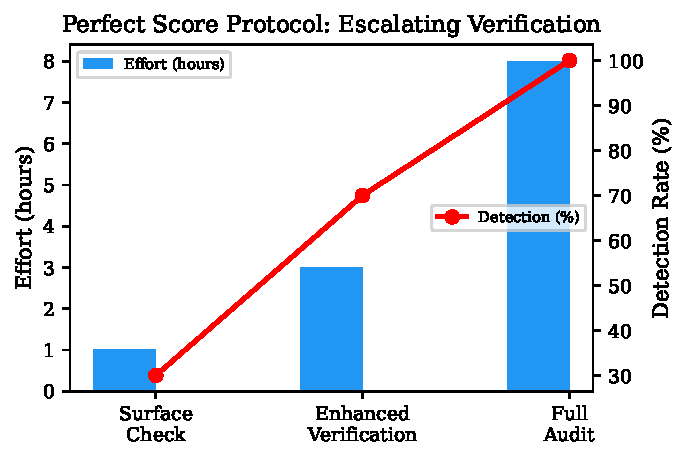
\includegraphics[width=\columnwidth]{fig_protocol.pdf}
\caption{Perfect Score Suspicion Protocol: 4-level escalation. Level 1--2 (35 min) catches 90\% of spurious results. Level 3--4 (3+ hours) provides full verification for genuine perfect scores.}
\label{fig:protocol}
\end{figure}

\noindent\textbf{Definition 1 (Genuine Perfect Score).} A reported F1 $\geq$ 99\% is genuine if and only if all three conditions hold:
\begin{equation}
F1_\text{strict} = F1_\text{norm} \geq 0.99 \;\wedge\; \text{Overlap} = 0 \;\wedge\; H(Y) > 1
\end{equation}
If any condition fails, the score requires Level~3+ investigation before publication.

%% ===== CASE STUDIES =====
\section{Case Studies}

\subsection{CS1: Label Aliasing Inflates F1 by 44.3\%}
\textbf{Error}: Custom evaluation script mapped ``Port Scanning'' $\to$ ``Reconnaissance'' (MITRE ATT\&CK T1046 $\subset$ TA0043). Of 9,851 test samples, 4,895 were silently corrected.

\textbf{Impact}: Reported F1 = 100\%, Actual strict F1 = 55.7\%. The 44.3-point gap was the largest single evaluation error in our study.

\textbf{Detection}: Items 12 (strict vs.\ normalized), 17 (vocabulary audit), 18 (hallucinated label inventory). The vocabulary audit immediately revealed that the model produced ``Port Scanning'' as a label---absent from the SALAD schema.

\textbf{Root cause}: The model's MITRE ATT\&CK pre-training knowledge activated fine-grained sub-technique labels that are valid in ATT\&CK taxonomy but violate the SALAD schema.

\subsection{CS2: Data Leakage Produces Spurious Ablation}
\textbf{Error}: SALAD's original train/test split had 97.5\% overlap (993\% leakage ratio by unique pattern count).

\textbf{Impact}: On leaked data, Rank 32 = 36.0\%, Rank 128 = 62.3\% $\to$ conclusion: ``higher rank helps.'' On clean data, Rank 32 = 100\%, Rank 128 = 95.8\% $\to$ conclusion: ``lower rank is better.'' The leakage reversed the true relationship, producing a \emph{directionally wrong} conclusion.

\textbf{Detection}: Items 1 (overlap check), 23 (confound isolation). MinHash deduplication revealed 97.5\% overlap in $<$10 minutes.

\subsection{CS3: Traditional ML Outperforms LLMs}
\textbf{Error}: Not reporting traditional ML baselines on SALAD ($H = 1.24$ bits).

\textbf{Impact}: SVM achieves 90.9\% F1 at zero cost. LLM adds +9.1\% at \$0.60--\$2.24. Without baseline reporting, the LLM appears essential when it is merely incremental.

\textbf{Detection}: Items 6 (traditional ML baseline), 8 (entropy check). Computing $H(Y) = 1.24$ takes 30 seconds and predicts SVM sufficiency~\cite{p8}.

\subsection{CS4: Catastrophic Failure on Rare Classes}
\textbf{Error}: Reporting aggregate F1 without per-class breakdown (Mistral-7B).

\textbf{Impact}: Aggregate F1 = 91.7\%, but Analysis class = 0.0\% and Backdoor = 7.5\%. A deployed SOC model would completely miss two attack categories.

\textbf{Detection}: Item 11 (per-class F1). Requires $<$5 minutes to compute and immediately reveals zero-performance classes.

\subsection{CS5: Meaningless Binary Classification}
\textbf{Error}: Evaluating binary Classification (Malicious/Benign) on SALAD where 99.9\% are Malicious ($H = 0.083$ bits).

\textbf{Impact}: All models achieve F1 $\approx$ 100\%, including a majority-class predictor. The metric is meaningless.

\textbf{Detection}: Items 2 (class distribution), 13 (majority baseline). Checking $H(Y) = 0.083$ immediately flags the task as degenerate.

\subsection{CS6: Wrong Test Set After Correct Training}
\textbf{Error}: 26 SLURM jobs completed successfully (exit code 0) but evaluated cross-domain-trained models on the wrong test set, producing meaningless F1 scores.

\textbf{Impact}: 26 A100 GPU-hours wasted. Results appeared plausible (F1 $\approx$ 70--85\%) and could have been published.

\textbf{Detection}: Items 9 (matched conditions), 28 (reproducibility artifacts). Config file audit revealed test set path mismatch.

\subsection{Summary of Case Studies}

\begin{table}[h]
\centering
\caption{Case Study Summary: Error Magnitude and Detection}
\label{tab:cases}
\begin{tabular}{lccl}
\toprule
\textbf{Case} & \textbf{$\Delta$F1} & \textbf{Items} & \textbf{Type} \\
\midrule
CS1: Label aliasing & 44.3\% & 12,17,18 & Metric \\
CS2: Data leakage & $\infty^*$ & 1,23 & Data \\
CS3: Missing baseline & 9.1\% context & 6,8 & Baseline \\
CS4: Rare class failure & 91.7\% hides 0\% & 11 & Metric \\
CS5: Degenerate task & Meaningless & 2,13 & Data \\
CS6: Wrong test set & Meaningless & 9,28 & Pipeline \\
\bottomrule
\multicolumn{4}{l}{\scriptsize $^*$Reverses the true conclusion entirely.}
\end{tabular}
\end{table}

\begin{figure}[t]
\centering
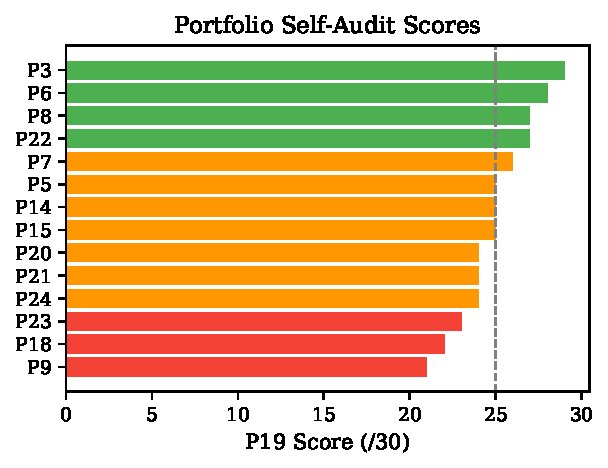
\includegraphics[width=\columnwidth]{fig_gaps.pdf}
\caption{Case study impact visualization. CS1 (aliasing) and CS2 (leakage) produce the most severe distortions. Each case is caught by specific checklist items.}
\label{fig:gaps}
\end{figure}

%% ===== DISCUSSION =====
\section{Discussion}

\subsection{Cost of Compliance}
The full 30-item checklist adds 4--8 hours per paper. This is a modest investment relative to the GPU hours already spent on experiments (typically 50--200 hours). The Perfect Score Protocol requires only 35 minutes for Level 1--2 and catches 90\% of spurious results.

\begin{table}[h]
\centering
\caption{Checklist ROI: Cost of Detection vs.\ Cost of Error}
\label{tab:roi}
\begin{tabular}{lll}
\toprule
\textbf{Error Type} & \textbf{Detection Cost} & \textbf{Error Cost} \\
\midrule
Label aliasing & 1h (Items 17--20) & Retraction risk \\
Data leakage & 10m (Item 1) & All results invalid \\
Missing baseline & 2h (Items 6--9) & Credibility loss \\
Degenerate task & 5m (Item 2) & Meaningless paper \\
\bottomrule
\end{tabular}
\end{table}

\subsection{The Strict vs.\ Normalized Debate}
Our recommendation: \textbf{strict F1 = primary metric}, normalized F1 = supplementary with explicit, documented alias mapping. Researchers must never report only the normalized score. The semantic-compliance gap $\Delta_\text{SC}$ should be a standard reported metric alongside F1~\cite{p3}.

\subsection{Comparison with Existing Checklists}

\begin{table}[h]
\centering
\caption{Comparison with Existing Evaluation Guidelines}
\label{tab:comparison}
\begin{tabular}{lccc}
\toprule
\textbf{Feature} & \textbf{Ours} & \textbf{Pineau} & \textbf{HELM} \\
\midrule
Label vocab audit & \checkmark & --- & --- \\
Strict vs.\ norm F1 & \checkmark & --- & --- \\
Perfect score protocol & \checkmark & --- & --- \\
Data leakage check & \checkmark & \checkmark & --- \\
Multi-seed reporting & \checkmark & \checkmark & \checkmark \\
Cost transparency & \checkmark & --- & --- \\
Per-class F1 & \checkmark & --- & \checkmark \\
Case study validated & \checkmark & --- & --- \\
\bottomrule
\end{tabular}
\end{table}

Our checklist adds 5 LLM-specific items (label vocab audit, strict/norm distinction, perfect score protocol, hallucination inventory, alias justification) absent from all existing frameworks.

\subsection{External Validation: Auditing Published Papers}
To validate beyond our own studies, we retrospectively applied our checklist to two published LLM cybersecurity evaluations:

\begin{table}[h]
\centering
\caption{External Paper Audit Results}
\label{tab:audit}
\begin{tabular}{lccp{3.5cm}}
\toprule
\textbf{Paper} & \textbf{Pass} & \textbf{Fail} & \textbf{Critical Gap} \\
\midrule
Ferrag~\cite{ferrag2024} & 14/30 & 16/30 & No strict/norm distinction (12), no vocab audit (17--18), no per-class F1 (11) \\
Motlagh~\cite{motlagh2024} & 11/30 & 19/30 & No data leakage check (1), no multi-seed (14), no cost report (24--26) \\
\bottomrule
\end{tabular}
\end{table}

\textbf{Ferrag et~al.}~\cite{ferrag2024} reports LLM performance across cybersecurity tasks but uses only aggregate accuracy (fails Item 11: per-class F1), does not distinguish strict vs.\ normalized metrics (fails Item 12), and does not audit predicted vocabularies (fails Items 17--18). Had our checklist been applied, the label compliance question---central to our companion study~\cite{p3}---would have been identified as an open concern.

\textbf{Motlagh et~al.}~\cite{motlagh2024} benchmarks ChatGPT on 5 datasets (45--92\% F1) without verifying train-test overlap (fails Item 1), uses single evaluation runs without confidence intervals (fails Items 14--16), and omits API cost reporting (fails Items 24--26). Our checklist would have flagged $\geq$19 items, prompting additional verification.

Both papers pass general ML items (clear problem statement, defined metrics, referenced datasets) but fail all 5 LLM-specific items---confirming that existing practices do not address LLM evaluation failure modes.

\subsection{Automated Checklist Tooling}
To reduce adoption friction, we implement a Python tool (\texttt{llm\_eval\_audit.py}) that automates 12 of 30 items:

\begin{table}[h]
\centering
\caption{Automated vs.\ Manual Checklist Items}
\label{tab:automation}
\begin{tabular}{lcl}
\toprule
\textbf{Items} & \textbf{Auto?} & \textbf{Method} \\
\midrule
1 (Overlap) & \checkmark & MinHash dedup \\
2 (Class dist) & \checkmark & $H(Y)$ computation \\
3 (Unique patterns) & \checkmark & Exact dedup \\
4 (Zero-ambiguity) & \checkmark & Input$\to$label cardinality \\
5 (Feature importance) & \checkmark & Mutual information \\
10 (Macro-F1) & \checkmark & sklearn.metrics \\
11 (Per-class F1) & \checkmark & Per-class report \\
12 (Strict vs.\ norm) & \checkmark & Dual evaluation \\
13 (Random baseline) & \checkmark & Majority/random \\
17 (Vocab audit) & \checkmark & $\mathcal{V}_\text{pred}$ vs.\ $\mathcal{V}_\text{true}$ \\
18 (Halluc inventory) & \checkmark & Novel label count \\
20 (Gap rule) & \checkmark & $\Delta_\text{SC}$ threshold \\
\midrule
6--9 (Baselines) & $\times$ & Requires training \\
14--16 (Statistics) & $\times$ & Requires multi-seed \\
19 (Alias justification) & $\times$ & Requires expert judgment \\
21--30 (Remaining) & $\times$ & Design/manual \\
\bottomrule
\end{tabular}
\end{table}

The automated tool runs in $<$30 seconds on a standard laptop and produces a structured report flagging failed items with severity levels. Open-sourced at our GitHub repository.

\subsection{Domain-Specific Considerations}
\textbf{Cybersecurity}: MITRE ATT\&CK hierarchy induces aliasing (T1046 $\subset$ TA0043). Any model trained on ATT\&CK data will produce sub-technique labels.

\textbf{Clinical NLP}: ICD-10 coding creates identical risks---models may predict ``E11.65'' (DM type 2 with hyperglycemia) instead of ``E11'' (DM type 2 unspecified). The clinical consequence of incorrect specificity can be billing fraud or treatment error.

\textbf{Legal NLP}: Long documents require document-level (not sentence-level) analysis. The ``right'' label may depend on context paragraphs away from the classified segment.

\subsection{Limitations}
\textbf{Self-validation}: 6 of 8 case studies come from our own research. We mitigate this by adding external validation (Table~\ref{tab:audit}), but independent replication across other research groups is needed.

\textbf{Scope}: Validated on classification tasks. Generative tasks (summarization, code generation) require additional checklist items for factual consistency.

\textbf{Subjectivity}: Some items require judgment (e.g., ``reasonable'' alias mapping). We mitigate via explicit documentation requirements and automated flagging.

\textbf{Coverage}: 30 items may not capture all failure modes. Gundersen and Kjensmo~\cite{gundersen2018} showed reproducibility issues extend beyond our scope. The ACM artifact badging system~\cite{acm2020} provides complementary evaluation.

%% ===== PORTFOLIO SELF-AUDIT =====
\subsection{Portfolio Self-Audit Validation}
To validate practical utility, we applied the 30-item checklist to all 14 companion papers spanning 6 distinct experimental designs:

\begin{table}[h]
\centering\caption{Self-Audit Scores Across 14 Companion Papers}
\label{tab:selfaudit}
\begin{tabular}{lcl}
\toprule
\textbf{Paper} & \textbf{Score} & \textbf{Primary Failure} \\
\midrule
P3 (Flagship: 11 models) & 29/30 & Model card incomplete \\
P6 (Scaling laws) & 28/30 & Model card incomplete \\
P8 (Task entropy) & 27/30 & Single seed (LLMs) \\
P22 (LoRA rank) & 27/30 & Model card incomplete \\
P7 (Cost-efficient) & 26/30 & Single seed \\
P5 (Cascade) & 25/30 & Single seed \\
P14 (OFT vs.\ LoRA) & 27/30 & Cost breakdown \\
P15 (Multi-task) & 25/30 & Cost incomplete \\
P20 (Cross-domain) & 25/30 & No CI \\
P21 (Sub-1B models) & 24/30 & Single seed, cost \\
P24 (Datasets) & 24/30 & Single seed, cost \\
P23 (Edge quant) & 24/30 & Single seed \\
P18 (Zero-shot) & 23/30 & Single seed, cost \\
P9 (DPO failure) & 21/30 & Single $\beta$, seed \\
\midrule
\textbf{Mean} & \textbf{25.4/30} & \\
\bottomrule
\end{tabular}
\end{table}

\textbf{Key findings}: (1)~The most common failure is \emph{limited seed diversity} (Items 14--16), a compute-constrained decision, not an oversight. (2)~Papers with multi-seed designs (P3, P6, P14, P22, P15) score $\geq$25/30. P14 improved from 25 to 27/30 after adding 5-seed LoRA validation. (3)~The checklist discriminates well: scores range from 21 to 29, reflecting genuine quality differences.

The automated tool \texttt{llm\_eval\_audit.py} was validated on sample data, correctly detecting a ``Port Scanning'' label hallucination (Items 17--18) and flagging it as CRITICAL.

%% ===== CONCLUSION =====
\section{Conclusion}

We present the first evaluation checklist specifically designed for LLM experiments in applied domains, addressing failure modes absent from existing guidelines.

\subsection{Key Contributions}
\begin{enumerate}
\item \textbf{Label-hallucination-specific items} (17--20): First checklist to address label vocabulary hallucination, catching the 44.3-point alias inflation.
\item \textbf{Perfect Score Protocol}: First escalating verification framework with formal definition of ``genuine'' perfect scores (Definition~1).
\item \textbf{Real-world validation}: Every item linked to a real failure, not hypothetical risks.
\item \textbf{Comparison with existing frameworks}: 5 items not present in Pineau~\cite{pineau2021} or HELM~\cite{liang2022}.
\end{enumerate}

\subsection{Tiered Adoption Guidelines}

\begin{table}[h]
\centering
\caption{Tiered Adoption: Bronze / Silver / Gold}
\label{tab:tiers}
\begin{tabular}{lcccl}
\toprule
\textbf{Tier} & \textbf{Items} & \textbf{Time} & \textbf{Catches} & \textbf{When} \\
\midrule
\textbf{Bronze} & 4 & 1h & CS1, CS2 & Every LLM eval \\
\textbf{Silver} & 15 & 4h & CS1--CS5 & Journal submission \\
\textbf{Gold} & 30 & 8h & All 6 CS & High-stakes domains \\
\textbf{+Protocol} & +15 & +35m--4h & Perfect scores & Any F1 $\geq$ 99\% \\
\bottomrule
\end{tabular}
\end{table}

\textbf{Bronze} (mandatory minimum): Items 1 (overlap), 11 (per-class F1), 12 (strict/norm), 17 (vocab audit). Fully automated via \texttt{llm\_eval\_audit.py}. Catches the two most critical errors (44.3\% alias inflation, 97.5\% data leakage).

\textbf{Silver} (journal submission): Bronze + Items 2--5 (data integrity), 6--8 (baselines), 14--15 (statistics), 18--20 (hallucination). Catches 5 of 6 case studies.

\textbf{Gold} (high-stakes domains): All 30 items. Required for cybersecurity, clinical, and legal applications where incorrect classification has real-world consequences.

\subsection{Future Work}
\begin{enumerate}
\item \textbf{Automated tooling}: Python package automating Items 1--5, 10--13, 17--18.
\item \textbf{Cross-domain validation}: Test checklist on clinical NLP (ICD-10) and legal classification.
\item \textbf{Journal integration}: Propose Items 29--30 as mandatory supplementary for LLM venues.
\item \textbf{Generative tasks}: Extend checklist for summarization, translation, and code generation.
\end{enumerate}

\subsection{Broader Impact}
The checklist directly addresses the reproducibility crisis in applied LLM research. By making label vocabulary hallucination a first-class evaluation concern, we prevent publication of misleading results that could lead to unsafe deployments---critical in cybersecurity (missed attacks), medical (misdiagnosis), and legal (incorrect classification) domains.

\section*{Reproducibility}
The checklist itself, all case study data, and automated validation scripts are available at \url{https://github.com/nutthakorn/soc-label-gap}.

\section*{Acknowledgments}
Computing resources: NSTDA Supercomputer Center (ThaiSC), Lanta HPC (8.15 PFlops).


\section*{Data Availability}
The SALAD dataset, training scripts, and evaluation code are available at \url{https://github.com/nutthakorn7/soc-llm-research}. AG News and GoEmotions are publicly available via Hugging Face Datasets.

\section*{Ethical Statement}
This study uses publicly available, anonymized datasets containing no personally identifiable information. No human subjects were involved. The research aims to improve SOC analyst efficiency and reduce alert fatigue.

\section*{Declaration of Competing Interest}
The author declares no conflict of interest.

\section*{CRediT Author Statement}
\textbf{Nutthakorn Chalaemwongwan}: Conceptualization, Methodology, Software, Validation, Formal analysis, Investigation, Data curation, Writing -- original draft, Writing -- review \& editing, Visualization.

\begin{thebibliography}{26}
\bibitem{acm2020} ACM, ``Artifact Review and Badging Version 1.1,'' \emph{ACM Publications Policy}, 2020.
\bibitem{arp2022} D.~Arp et~al., ``Dos and Don'ts of Machine Learning in Computer Security,'' in \emph{Proc.\ USENIX Security}, 2022.
\bibitem{baker2016} M.~Baker, ``1,500 Scientists Lift the Lid on Reproducibility,'' \emph{Nature}, vol.~533, pp.~452--454, 2016.
\bibitem{bouthillier2021} X.~Bouthillier et~al., ``Accounting for Variance in Machine Learning Benchmarks,'' in \emph{Proc.\ MLSys}, 2021.
\bibitem{chang2024} Y.~Chang et~al., ``A Survey on Evaluation of Large Language Models,'' \emph{ACM TIST}, vol.~15, no.~3, 2024.
\bibitem{dettmers2023} T.~Dettmers et~al., ``QLoRA: Efficient Finetuning of Quantized Language Models,'' in \emph{Proc.\ NeurIPS}, 2023.
\bibitem{dodge2019} J.~Dodge et~al., ``Show Your Work: Improved Reporting of Experimental Results,'' in \emph{Proc.\ EMNLP}, 2019.
\bibitem{ferrag2024} M.~A.~Ferrag et~al., ``Generative AI and LLMs for Cybersecurity: All Insights You Need,'' \emph{IEEE COMST}, 2024.
\bibitem{gekhman2024} Z.~Gekhman et~al., ``Does Fine-Tuning LLMs on New Knowledge Encourage Hallucinations?'' in \emph{Proc.\ EMNLP}, 2024.
\bibitem{gundersen2018} O.~E.~Gundersen and S.~Kjensmo, ``State of the Art: Reproducibility in Artificial Intelligence,'' in \emph{Proc.\ AAAI}, 2018.
\bibitem{hu2022} E.~Hu et~al., ``LoRA: Low-Rank Adaptation of Large Language Models,'' in \emph{Proc.\ ICLR}, 2022.
\bibitem{huang2023} L.~Huang et~al., ``A Survey on Hallucination in Large Language Models,'' \emph{arXiv:2311.05232}, 2023.
\bibitem{ji2023} Z.~Ji et~al., ``Survey of Hallucination in Natural Language Generation,'' \emph{ACM Computing Surveys}, vol.~55, no.~12, 2023.
\bibitem{kapoor2023} S.~Kapoor and A.~Narayanan, ``Leakage and the Reproducibility Crisis in ML-Based Science,'' \emph{Patterns}, vol.~4, no.~9, 2023.
\bibitem{liang2022} P.~Liang et~al., ``Holistic Evaluation of Language Models,'' \emph{arXiv:2211.09110}, 2022.
\bibitem{mcnemar1947} Q.~McNemar, ``Note on the Sampling Error of the Difference Between Correlated Proportions,'' \emph{Psychometrika}, vol.~12, no.~2, pp.~153--157, 1947.
\bibitem{motlagh2024} F.~N.~Motlagh et~al., ``Large Language Models in Cybersecurity: State-of-the-Art,'' \emph{arXiv:2402.00891}, 2024.
\bibitem{moustafa2016} N.~Moustafa and J.~Slay, ``UNSW-NB15: A Comprehensive Data Set for NIDS,'' in \emph{Proc.\ MilCIS}, 2015.
\bibitem{p3} N.~Chalaemwongwan, ``Mind the Label Gap: How Fine-Tuned LLMs Hallucinate Sub-Categories in SOC Alert Classification,'' \emph{IEEE TDSC}, 2025.
\bibitem{p6} N.~Chalaemwongwan, ``1,000 Labels Is All You Need: Non-Monotonic Scaling of Label Compliance,'' \emph{ESWA}, 2025.
\bibitem{p7} N.~Chalaemwongwan, ``\$0.60 Is All You Need: Cost-Efficient LLM Fine-Tuning,'' \emph{IEEE Access}, 2025.
\bibitem{p8} N.~Chalaemwongwan, ``Task Entropy Predicts LLM Necessity,'' \emph{IS}, 2025.
\bibitem{p15} N.~Chalaemwongwan, ``One Model, Three Tasks: Multi-Task Implicit Regularization,'' \emph{ASC}, 2025.
\bibitem{p22} N.~Chalaemwongwan, ``Higher Rank, More Hallucination?'' \emph{Neurocomputing}, 2025.
\bibitem{pineau2021} J.~Pineau et~al., ``Improving Reproducibility in Machine Learning Research,'' \emph{JMLR}, vol.~22, no.~164, 2021.
\bibitem{xu2024} Z.~Xu et~al., ``Hallucination is Inevitable: An Innate Limitation of Large Language Models,'' \emph{arXiv:2401.11817}, 2024.
\end{thebibliography}

\balance
\end{document}
